% Ein -*-latex-*- File


\newsavebox{\lotte}
\sbox{\lotte}{\mbox{}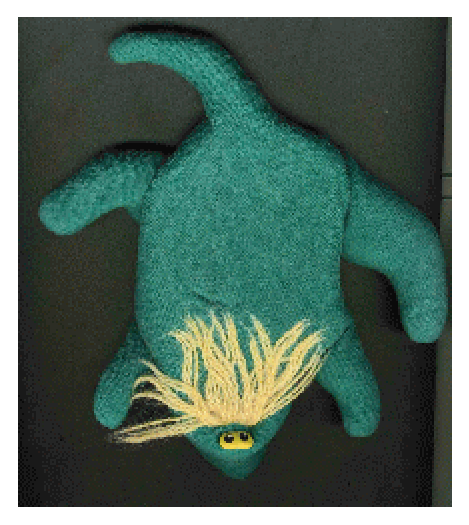
\includegraphics{Lotte.ps}}
\newlength{\lottebreite}
\newlength{\lotteplatz}
\settowidth{\lottebreite}{\usebox{\lotte}}
\setlength{\lotteplatz}{\textwidth}
\addtolength{\lotteplatz}{-\lottebreite}

\noindent
\usebox{\lotte}
\hfill
\begin{minipage}[b]{0.95\lotteplatz}

\addsec{Lotte}

Mau! 

Ich bin Lotte, Tilmans katzengr�ne Katze. Ich h�nge gerne in H�rs�len
herum, kann sehr gut Yoga und f�hle mich manchmal ein bisschen
schlapp\dots\\
Die kommenden zwei Semester werde ich allerdings mit Tilman zusammen
in Dub"-lin verbringen.
\end{minipage}

\vspace{2ex}
\noindent
Inzwischen hab ich auch eine eigene Homepage bei der FaNatIk in
Bielefeld.%
\footnote{\texttt{http://www.techfak.uni-bielefeld.de/techfak/fachschaft/leute/Lotte/}}

\noindent
Und hier f�r die, die etwas �ber meinen Stoff-Wechsel oder meine
Gen�htik wissen m�chten:

\mbox{}
\hfill
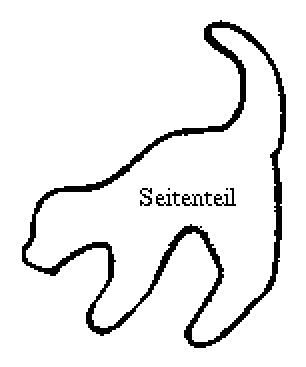
\includegraphics{lottechen-seite.ps} 
\hfill
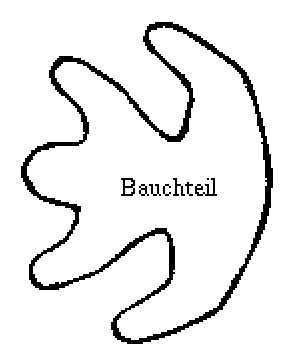
\includegraphics{lottechen-unten.ps} 
\hfill
\mbox{}

Gr�ne Katzen vermehren sich subversiv. Sie sehen s�� aus und hoffen,
da� jemand eine n�ht. Das nennt man Gen�hse (kurz f�r "`Geh, n�h sie"').

Wer selbst eine gr�ne Katze haben m�chte, kaufe ein gutes St�ck
katzengr�nen Nicki-Stoff, n�he einen Bodenschnitt und je einen
Seitenschnitt in beiden Orientierungen zusammen (L�nge Kopf-Schwanz
etwa 25 cm), knete aus gelbem, schwarzem und wei�em Fimo Augen, ziehe
ein B�schel gelber Wolle als Haare in den Kopf und f�lle die so
entstehende gr�ne Katze mit Plastikgranulat (gibt's alles in
Bastelgesch�ften zu kaufen).\hfill\textit{Tilman Vierhuff, 1997-5-27}


